\section{Data-driven results for the 2D SWE}\label{sec:data-driven-results-2D}
In this section we present the results for the 2D SWE using data-driven models. 
The initial condition, a Gaussian function, is the same as in the 1D case but extended to two dimensions.
We the 2D SWE using both a CNN and and FNO model, comparing their performance in terms of run time and accuracy.
Additionally, we compare their run time to the FVM to evaluate whether the data-driven models can serve as a faster alternative.
We also assess the models' ability to generalize to a finer grid by training them on a coarse grid and making predictions of a fine grid.
Finally, we evaluate the models' capability to generalize further in time, testing their long-term predictive performance.

The initial condition for the 2D problem is a Gaussian function as given in~\eqref{eq:2D_swe_ic_gaussian}.
The initial condition is illustrated in \autoref{fig:2D_gauss_initial_condition}.
\begin{figure}[H]
    \centering
    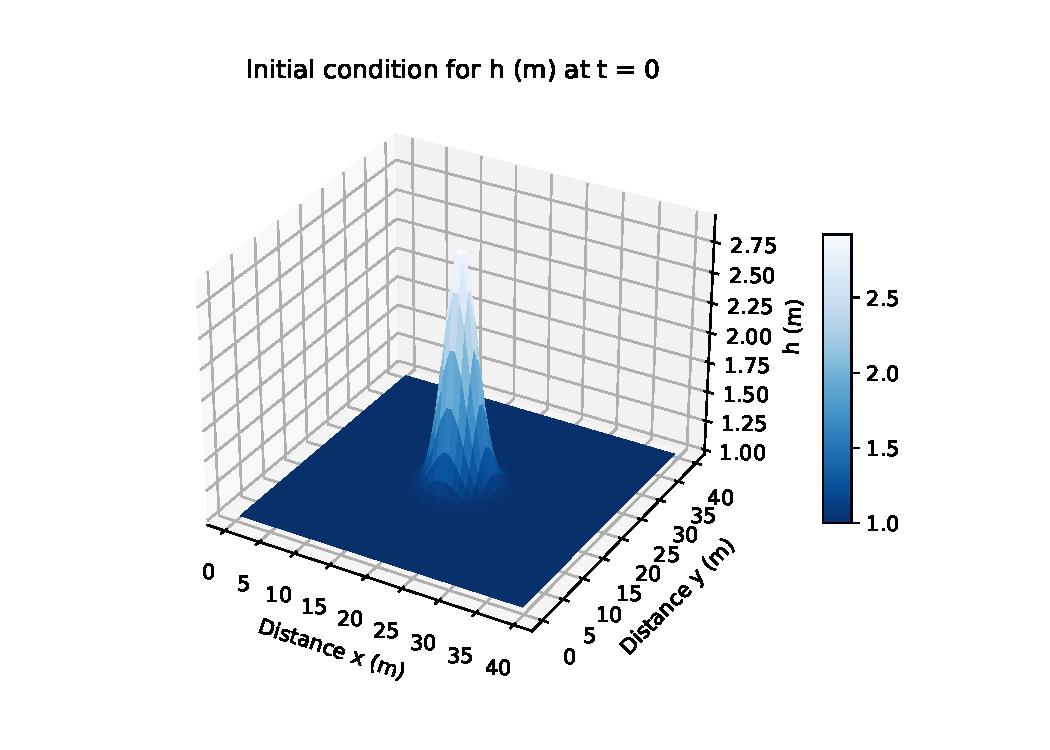
\includegraphics[width=0.8\textwidth]{C:/Users/Matteo/Shallow-Water-Equations/plots/2D_gauss_initial_condition.pdf}
    \caption{Initial condition for the 2D SWE.}\label{fig:2D_gauss_initial_condition}
\end{figure}
In \autoref{fig:2D_gauss_initial_condition} we see the initial condition for the 2D SWE problem, which is close to the 2D dam break problem, only here with a Gaussian function.
The solution is generated from $t = 0$ to $t = 5$ s.
Some information of the data used for the 2D SWE generated by the FVM can be found in \autoref{tab:data_2D_SWE}.
\begin{table}[H]
    \centering
    \begin{tabular}{c|ccccc}
        \textbf{Case} & \textbf{n\_train} & \textbf{n\_val} & \textbf{n\_test} & $\mathbf{\Delta x}$ & $\mathbf{\Delta t}$ \\
        \hline
        2D SWE, N = 64 & 48 & 16 & 17 & 0.625 m  & $[0.050 \text{ s}, 0.073 \text{ s}]$ \\
        2D SWE, N = 128 & 99 & 33 & 33 & 0.3125 m  & $[0.025 \text{ s}, 0.035 \text{ s}]$ \\
    \end{tabular}
    \caption{Details of the used data for the case with the 2D SWE for both a number of grid points $N=64$ and $N=128$.}\label{tab:data_2D_SWE}
\end{table}
In \autoref{tab:data_2D_SWE} we see that the train/validation/test data split is $60\%/20\%/20\%$ for both $N = 64$ and $N = 128$.
In the FVM we use a variable time step size $\Delta t$ to ensure stability, which is why the time step size varies.
We see that for $N = 64$ the time step size varies between $0.050$ s and $0.073$ s, while for $N = 128$ the time step size varies between $0.025$ s and $0.035$ s.
The time step size for the higher $N$ is in general smaller than for the lower $N$ to ensure stability.
This is also what gives more data points for $N = 128$ compared to $N = 64$.


\subsubsection*{CNN Model}
We train a CNN model with several convolutional layers and ReLU activation functions.
We use the Adam optimizer with a learning rate of $0.001$ and a batch size of $32$.
The model is trained on the data for $60\%$ of the time steps, validated on $20\%$ of the time steps, and tested on the last $20\%$ of the time steps.
We make predictions from $t = 0$ to $t = 5$.
The model is trained for $500$ epochs.
The training and validation loss for the 2D CNN model can be seen in \autoref{fig:2D_CNN_loss}.
\begin{figure}[H]
    \centering
    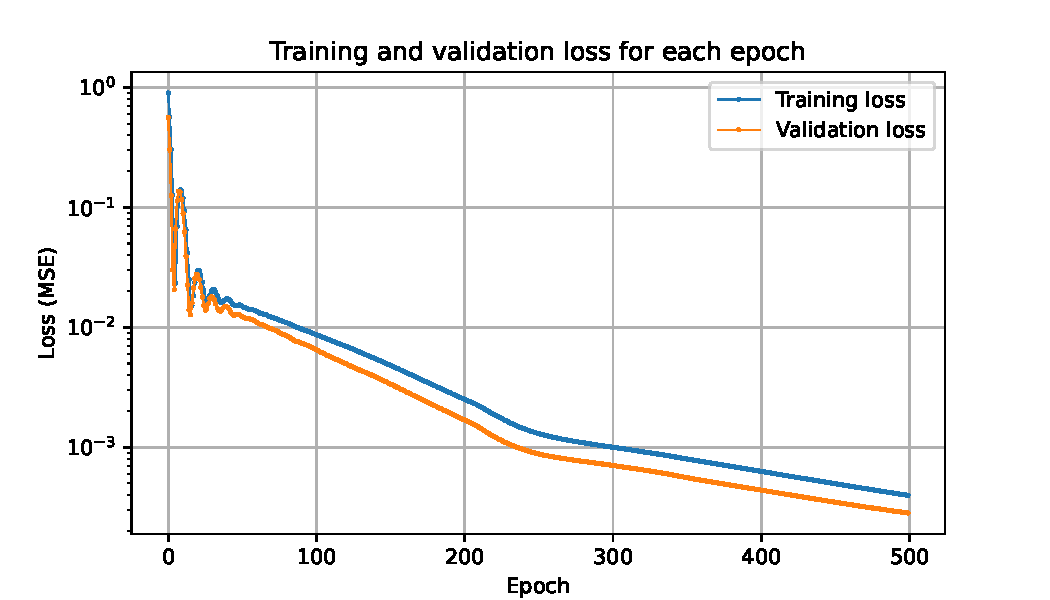
\includegraphics[width=0.7\textwidth]{C:/Users/Matteo/Shallow-Water-Equations/plots/2D_CNN_loss.pdf}
    \caption{Training and validation loss for the 2D CNN model.}\label{fig:2D_CNN_loss}
\end{figure}
\autoref{fig:2D_CNN_loss} shows that the training and validation loss are decreasing, as a function of the number of epochs.
The error plot for the last prediction for the 2D CNN can be seen in \autoref{fig:2D_CNN_error}.
\begin{figure}[H]
    \centering
    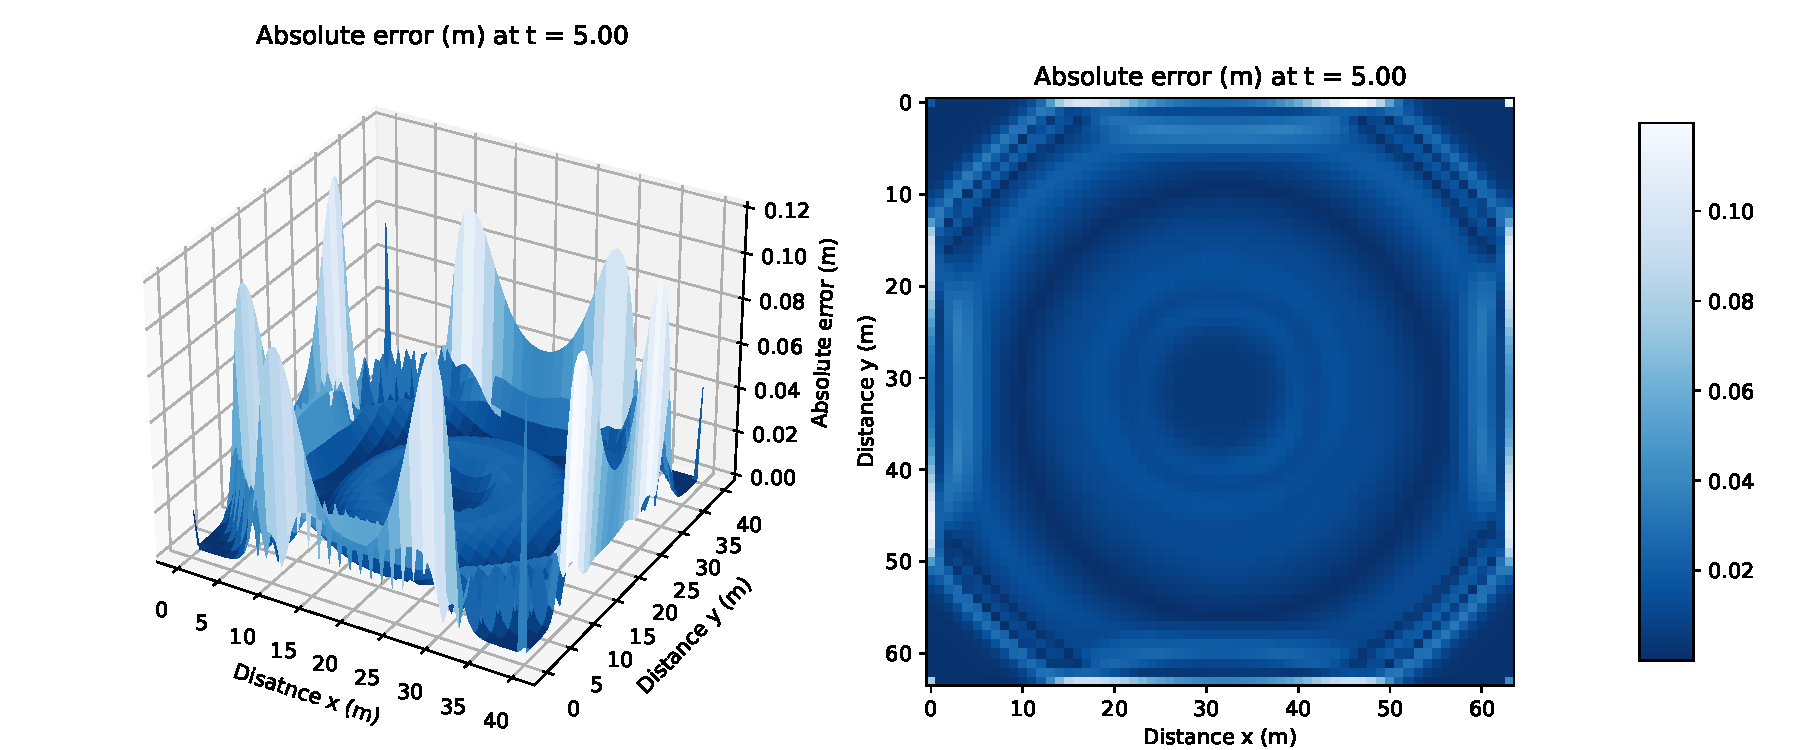
\includegraphics[width=0.8\textwidth]{C:/Users/Matteo/Shallow-Water-Equations/plots/2D_CNN_error.pdf}
    \caption{Error plot for the last prediction for the 2D CNN.}\label{fig:2D_CNN_error}
\end{figure}
From \autoref{fig:2D_CNN_error}, we see that overall the absolute error is small, meaning that the CNN model is able to learn the dynamics of solution.
The error is largest at the boundaries. 
This may be due to the fact that in this case we are working with boundary conditions simulating a wall.
Hence, when the wave hits the wall, the wave is reflected, and the model has to learn the reflection of the wave.
This may also lead to discontinuities in the solution, which can be difficult for the model to handle.

\subsubsection*{FNO Model}
We train a FNO model with the same training/validation/testing split as for the CNN model.
The FNO model uses 8 Fourier modes, the Adam optimizer with a learning rate of $0.001$, and a batch size of $10$.
The model is trained for $500$ epochs.
The training and validation loss for the 2D FNO model can be seen in \autoref{fig:2D_FNO_loss}.
\begin{figure}[H]
    \centering
    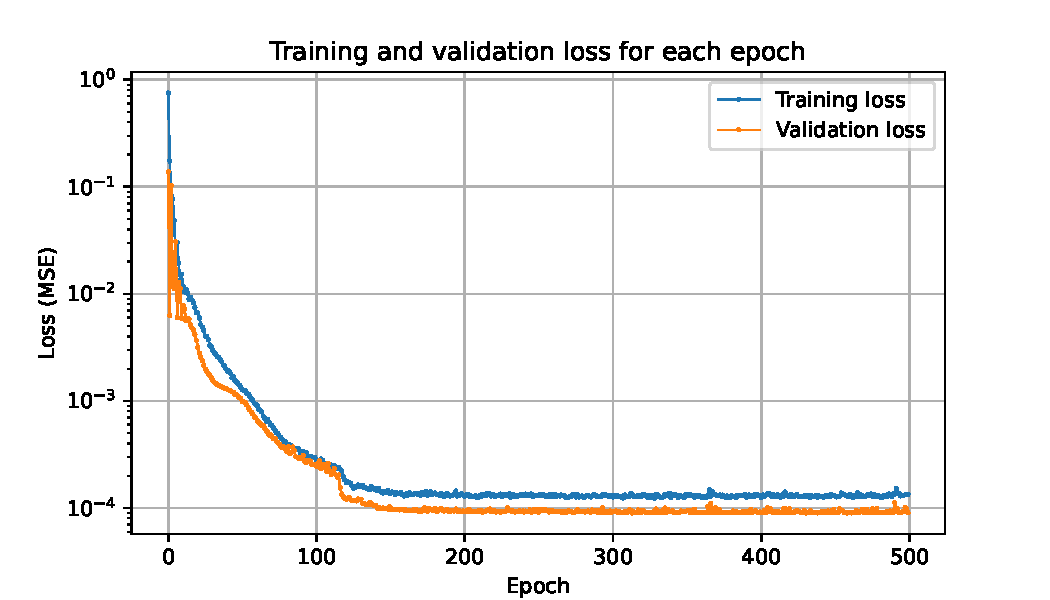
\includegraphics[width=0.8\textwidth]{C:/Users/Matteo/Shallow-Water-Equations/plots/2D_FNO_loss.pdf}
    \caption{Training and validation loss for the 2D FNO model.}\label{fig:2D_FNO_loss}
\end{figure}
From \autoref{fig:2D_FNO_loss} we see that the training and validation loss are decreasing, and more or less stable with some fluctations. 
The plot suggests that the model has converged.
The error plot for the last prediction for the 2D FNO can be seen in \autoref{fig:2D_FNO_error}.
\begin{figure}[H]
    \centering
    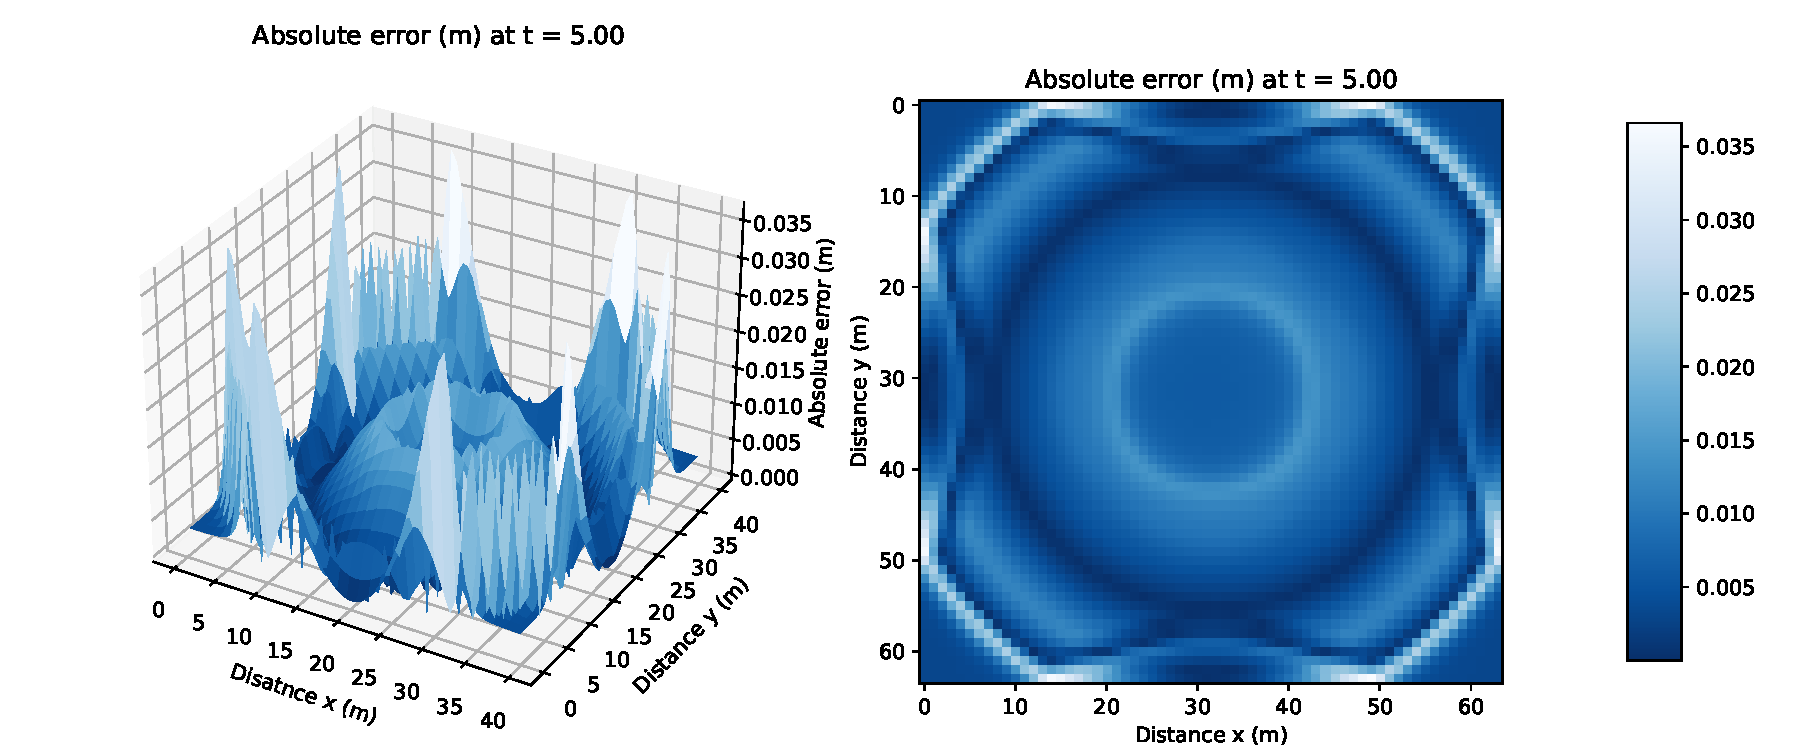
\includegraphics[width=0.8\textwidth]{C:/Users/Matteo/Shallow-Water-Equations/plots/2D_FNO_error.pdf}
    \caption{Error plot for the last prediction for the 2D FNO.}\label{fig:2D_FNO_error}
\end{figure}
As for the CNN model, the error is largest at the boundaries.
However, we notice that the absolute error is smaller for the FNO model compared to the CNN model.

\subsubsection*{Comparison}
We compare the performance of the CNN and FNO models in terms of the MSE and MAE for the predictions.
We test for both $N = 64$ and $N = 128$ grid points in each direction.
The errors are calculated for the test data, i.e., the last $20\%$ of the time steps.
The results are summarized in \autoref{tab:results_2D_comparison}, together with the time for training the models.
\begin{table}[H]
    \centering
    \small % Reduce font size
    \begin{tabular}{c|cccc|cccc}
        Model & \multicolumn{4}{c|}{$N = 64$} & \multicolumn{4}{c}{$N = 128$} \\
        \cline{2-9}
        & Epochs & MSE & MAE & Time (s) & Epochs & MSE & MAE & Time (s) \\
        \hline
        CNN  &
        \input{C:/Users/Matteo/Shallow-Water-Equations/saved_results/2D_CNN_Nx=64_nepochs.txt} &
        \input{C:/Users/Matteo/Shallow-Water-Equations/saved_results/2D_CNN_Nx=64_MSE_test.txt} & 
        \input{C:/Users/Matteo/Shallow-Water-Equations/saved_results/2D_CNN_Nx=64_MAE_test.txt} &
        \input{C:/Users/Matteo/Shallow-Water-Equations/saved_results/2D_CNN_Nx=64_time.txt} &
        \input{C:/Users/Matteo/Shallow-Water-Equations/saved_results/2D_CNN_Nx=128_nepochs.txt} &
        \input{C:/Users/Matteo/Shallow-Water-Equations/saved_results/2D_CNN_Nx=128_MSE_test.txt} &
        \input{C:/Users/Matteo/Shallow-Water-Equations/saved_results/2D_CNN_Nx=128_MAE_test.txt} &
        \input{C:/Users/Matteo/Shallow-Water-Equations/saved_results/2D_CNN_Nx=128_time.txt} 
        \\
        \hline
        FNO  &
        \input{C:/Users/Matteo/Shallow-Water-Equations/saved_results/2D_FNO_Nx=64_nepochs.txt} &
        \input{C:/Users/Matteo/Shallow-Water-Equations/saved_results/2D_FNO_Nx=64_MSE_test.txt} &
        \input{C:/Users/Matteo/Shallow-Water-Equations/saved_results/2D_FNO_Nx=64_MAE_test.txt} &
        \input{C:/Users/Matteo/Shallow-Water-Equations/saved_results/2D_FNO_Nx=64_time.txt} &
        \input{C:/Users/Matteo/Shallow-Water-Equations/saved_results/2D_FNO_Nx=128_nepochs.txt} &
        \input{C:/Users/Matteo/Shallow-Water-Equations/saved_results/2D_FNO_Nx=128_MSE_test.txt} &
        \input{C:/Users/Matteo/Shallow-Water-Equations/saved_results/2D_FNO_Nx=128_MAE_test.txt} &
        \input{C:/Users/Matteo/Shallow-Water-Equations/saved_results/2D_FNO_Nx=128_time.txt}
        \\
        \hline
    \end{tabular}
    \caption{Test loss in terms of MSE and MAE, and time for training the models for the 2D SWE.}\label{tab:results_2D_comparison}
\end{table}
We see that the FNO model in general needs fewer epochs to converge compared to the CNN model, but it also takes longer time to train.
From the theory we know that FNO are supposed to work when we are training on a coarse grid and then make predictions on a fine grid.
To test this, we will train the models on a coarse grid and then make predictions on a fine grid.
The table below shows the results when the models are trained on a grid with $N = 64$ and subsequently making predictions on a finer grid with $N = 128$.
\begin{table}[H]
    \centering
    \begin{tabular}{c|ccccc}
        Model & \multicolumn{5}{c}{$N = 128$} \\
        \cline{2-6}
        & Epochs & MSE & MAE & Training time (s) & Prediction time (s) \\
        \hline
        CNN &
        \input{C:/Users/Matteo/Shallow-Water-Equations/saved_results/2D_CNN_train_Nx=64_test_N=128_nepochs.txt} &
        \input{C:/Users/Matteo/Shallow-Water-Equations/saved_results/2D_CNN_train_Nx=64_test_N=128_MSE_test.txt} &
        \input{C:/Users/Matteo/Shallow-Water-Equations/saved_results/2D_CNN_train_Nx=64_test_N=128_MAE_test.txt} &
        \input{C:/Users/Matteo/Shallow-Water-Equations/saved_results/2D_CNN_train_Nx=64_test_N=128_train_time.txt} &
        \input{C:/Users/Matteo/Shallow-Water-Equations/saved_results/2D_CNN_train_Nx=64_test_N=128_time.txt} \\
        FNO  &
        \input{C:/Users/Matteo/Shallow-Water-Equations/saved_results/2D_FNO_train_Nx=64_test_N=128_nepochs.txt} &
        \input{C:/Users/Matteo/Shallow-Water-Equations/saved_results/2D_FNO_train_Nx=64_test_N=128_MSE_test.txt} &
        \input{C:/Users/Matteo/Shallow-Water-Equations/saved_results/2D_FNO_train_Nx=64_test_N=128_MAE_test.txt} &
        \input{C:/Users/Matteo/Shallow-Water-Equations/saved_results/2D_FNO_train_Nx=64_test_N=128_train_time.txt} &
        \input{C:/Users/Matteo/Shallow-Water-Equations/saved_results/2D_FNO_train_Nx=64_test_N=128_time.txt} 
    \end{tabular}
    \caption{Test loss in terms of MSE and MAE, and time for training the FNO model on a grid with $N = 64$ and then making predictions on a grid with $N = 128$.}\label{tab:results_2D_train_64_test_128}
\end{table}
From the results in \autoref{tab:results_2D_train_64_test_128} we see that the errors for the FNO model are small, meaning that the FNO model is able to generalize to a finer grid.
The CNN model has a higher error and if it is accurate enough depends on the application.
This way, it is possible to train the FNO model on a coarse grid and then make predictions on a fine grid, which is a great advantage when solving the SWE numerically, as it is very computationally expensive to solve the SWE on a fine grid using the FVM.
By comparing the run time of the FVM, see \autoref{tab:scalability}, we observe that the data-driven models offer an alternative, which may be advantageous depending on the specific application.
This approach provides a potential solution to the scalability challenges we are facing when solving the SWE numerically.
To test this ability further, we will train the models on a grid with $N = 64$ and then make predictions on a grid with $N = 256$.
The results are summarized in \autoref{tab:results_2D_train_64_test_256}.
\begin{table}[H]
    \centering
    \begin{tabular}{c|ccccc}
        Model & \multicolumn{5}{c}{$N = 256$} \\
        \cline{2-6}
        & Epochs & MSE & MAE & Training time (s) & Prediction time (s) \\
        \hline
        CNN &
        \input{C:/Users/Matteo/Shallow-Water-Equations/saved_results/2D_CNN_train_Nx=64_test_N=256_nepochs.txt} &
        \input{C:/Users/Matteo/Shallow-Water-Equations/saved_results/2D_CNN_train_Nx=64_test_N=256_MSE_test.txt} &
        \input{C:/Users/Matteo/Shallow-Water-Equations/saved_results/2D_CNN_train_Nx=64_test_N=256_MAE_test.txt} &
        \input{C:/Users/Matteo/Shallow-Water-Equations/saved_results/2D_CNN_train_Nx=64_test_N=256_train_time.txt} &
        \input{C:/Users/Matteo/Shallow-Water-Equations/saved_results/2D_CNN_train_Nx=64_test_N=256_time.txt} \\
        FNO  &
        \input{C:/Users/Matteo/Shallow-Water-Equations/saved_results/2D_FNO_train_Nx=64_test_N=256_nepochs.txt} &
        \input{C:/Users/Matteo/Shallow-Water-Equations/saved_results/2D_FNO_train_Nx=64_test_N=256_MSE_test.txt} &
        \input{C:/Users/Matteo/Shallow-Water-Equations/saved_results/2D_FNO_train_Nx=64_test_N=256_MAE_test.txt} &
        \input{C:/Users/Matteo/Shallow-Water-Equations/saved_results/2D_FNO_train_Nx=64_test_N=256_train_time.txt} &
        \input{C:/Users/Matteo/Shallow-Water-Equations/saved_results/2D_FNO_train_Nx=64_test_N=256_time.txt} 
    \end{tabular}
    \caption{Test loss in terms of MSE and MAE, and time for training the FNO model on a grid with $N = 64$ and then making predictions on a grid with $N = 256$.}\label{tab:results_2D_train_64_test_256}
\end{table}
The results in \autoref{tab:results_2D_train_64_test_256} show that the FNO model is able to generalize to a grid with $N = 256$.
While the errors are a bit higher than for the predictions on a grid with $N = 128$, the errors are still small, and for many applications the errors may be acceptable.
The results for the CNN model are not as good as for the FNO model, but the CNN model is still, to some extent, able to generalize to a finer grid.

\subsubsection*{Long-term predictions}
We are particularly interested in evaluating the models' ability to generalize further in time.
To do this we train the model on the generated 2D data with a fixed time step size of $\Delta t = 0.025$.
To test this, we will train the models on a time interval $[0, 5]$ and make predictions for up to $n = 200$ time steps in the future, equivalent predicting up to $t = 10$ s.

Initially, we adopted an iterative approach, where the model made a prediction for the next time step and used that prediction as input for the next time step.
While this approach produces acceptable results for the inital time steps, the error increases as we make predictions further in time, probably due to accumulating errors.
To address this issue, we implemented an alternative approach by creating sequences of data and training the model to predict the next time step based on the entire sequence.
In this method, the most recent prediction becomes part of a sequence, distributing the influence across subsequent predictions, rather than heavily impacting the next prediction alone.
This approach aims to stabilize long-term predictions.
The error plot for the long-term predictions from the CNN model can be seen in \autoref{fig:2D_CNN_long_term_error}.
\begin{figure}[H]
    \centering
    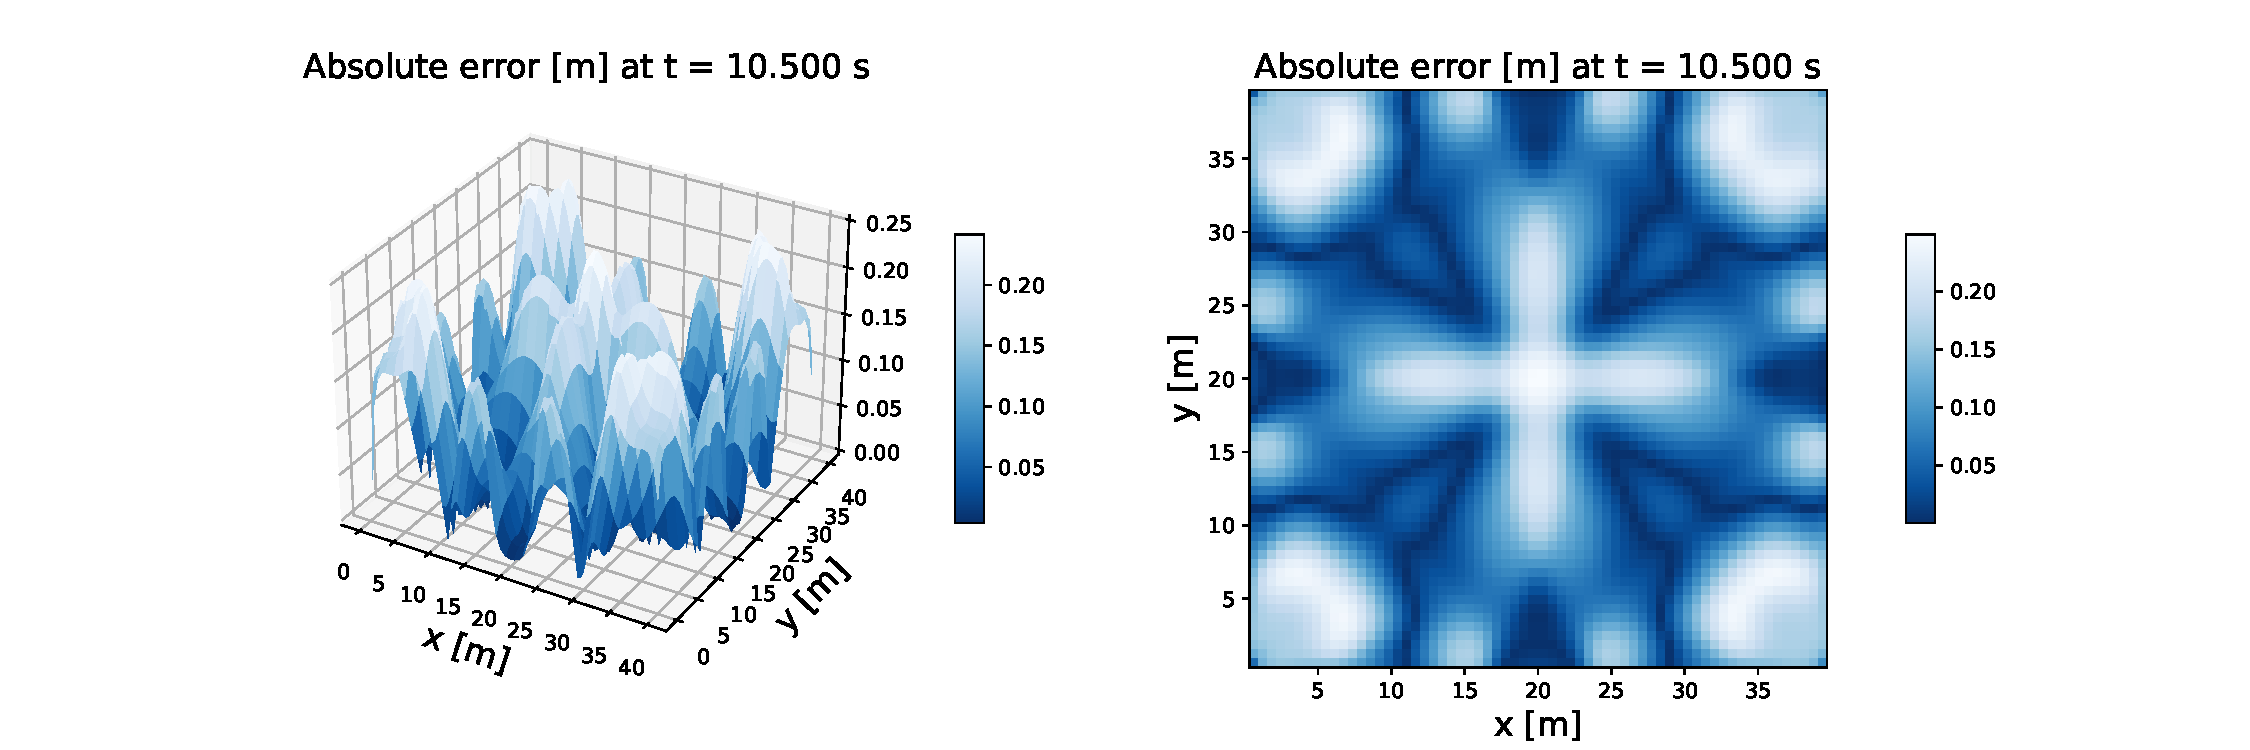
\includegraphics[width=\textwidth]{C:/Users/Matteo/Shallow-Water-Equations/plots/2D_CNN_long_term_predictions_error_Ntrain=64_Npred=64_idx=20.pdf}
    \caption{Error plot for the long-term prediction for the 2D CNN model.}\label{fig:2D_CNN_long_term_error}
\end{figure}
\autoref{fig:2D_CNN_long_term_error} shows that the error is larger for the short-term predictions in \autoref{fig:2D_CNN_error} compared to the long-term predictions.
But it has not increased drastically.
We run the same test for the FNO model.
The error plots of the long-term predictions from the FNO model after 20 time steps, equivalent to $t = 0.5$ s, can be seen in \autoref{fig:2D_FNO_long_term_error}.
\begin{figure}[H]
    \centering
    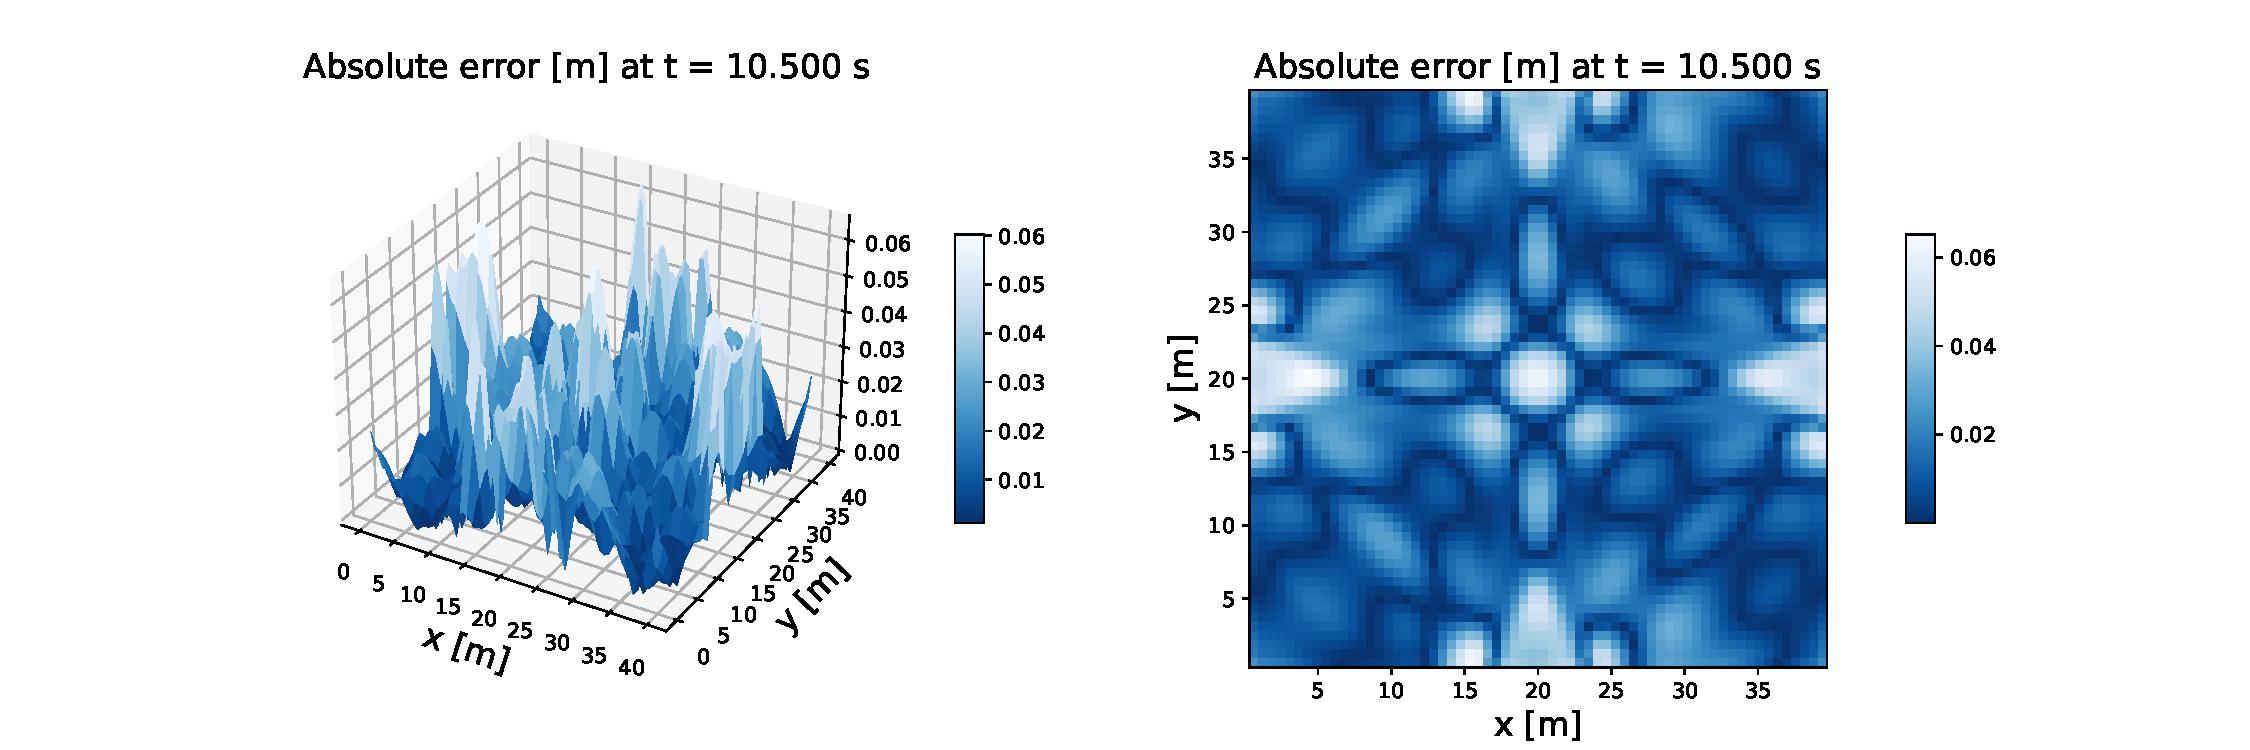
\includegraphics[width=\textwidth]{C:/Users/Matteo/Shallow-Water-Equations/plots/2D_FNO_long_term_predictions_error_Ntrain=64_Npred=64_idx=20.pdf}
    \caption{Error plot for the long-term prediction for the 2D FNO model.}\label{fig:2D_FNO_long_term_error}
\end{figure}
From the error plot in \autoref{fig:2D_FNO_long_term_error}, we see that the error is bigger than for the short-term predictions in \autoref{fig:2D_FNO_error}, but for many applications still acceptable.
We also see that error for the FNO model is smaller than for the CNN model, indicating that the FNO model is able to generalize further in time and make long-term predictions.
A plot of the predictions and the ground truth can be found in \autoref{fig:2D_FNO_long_term_predictions} in Appendix \autoref{app:2D_SWE_long_term_prediction}.
The corresponding error plot for $n = 40$ time steps can be seen in \autoref{fig:2D_FNO_long_term_error_40} in Appendix \autoref{app:2D_SWE_long_term_prediction}, where we see that the error has increased.

To get an overview of how the model performs over time, we plot the error in each time step for the long-term prediction for up to $n = 200$ time steps in the future.
To compare the error we have plotted the MSE, MAE and the max error for the long-term predictions for the CNN and FNO models in \autoref{fig:2D_CNN_FNO_mse_mae_max_error}.
\begin{figure}[H]
    \centering
    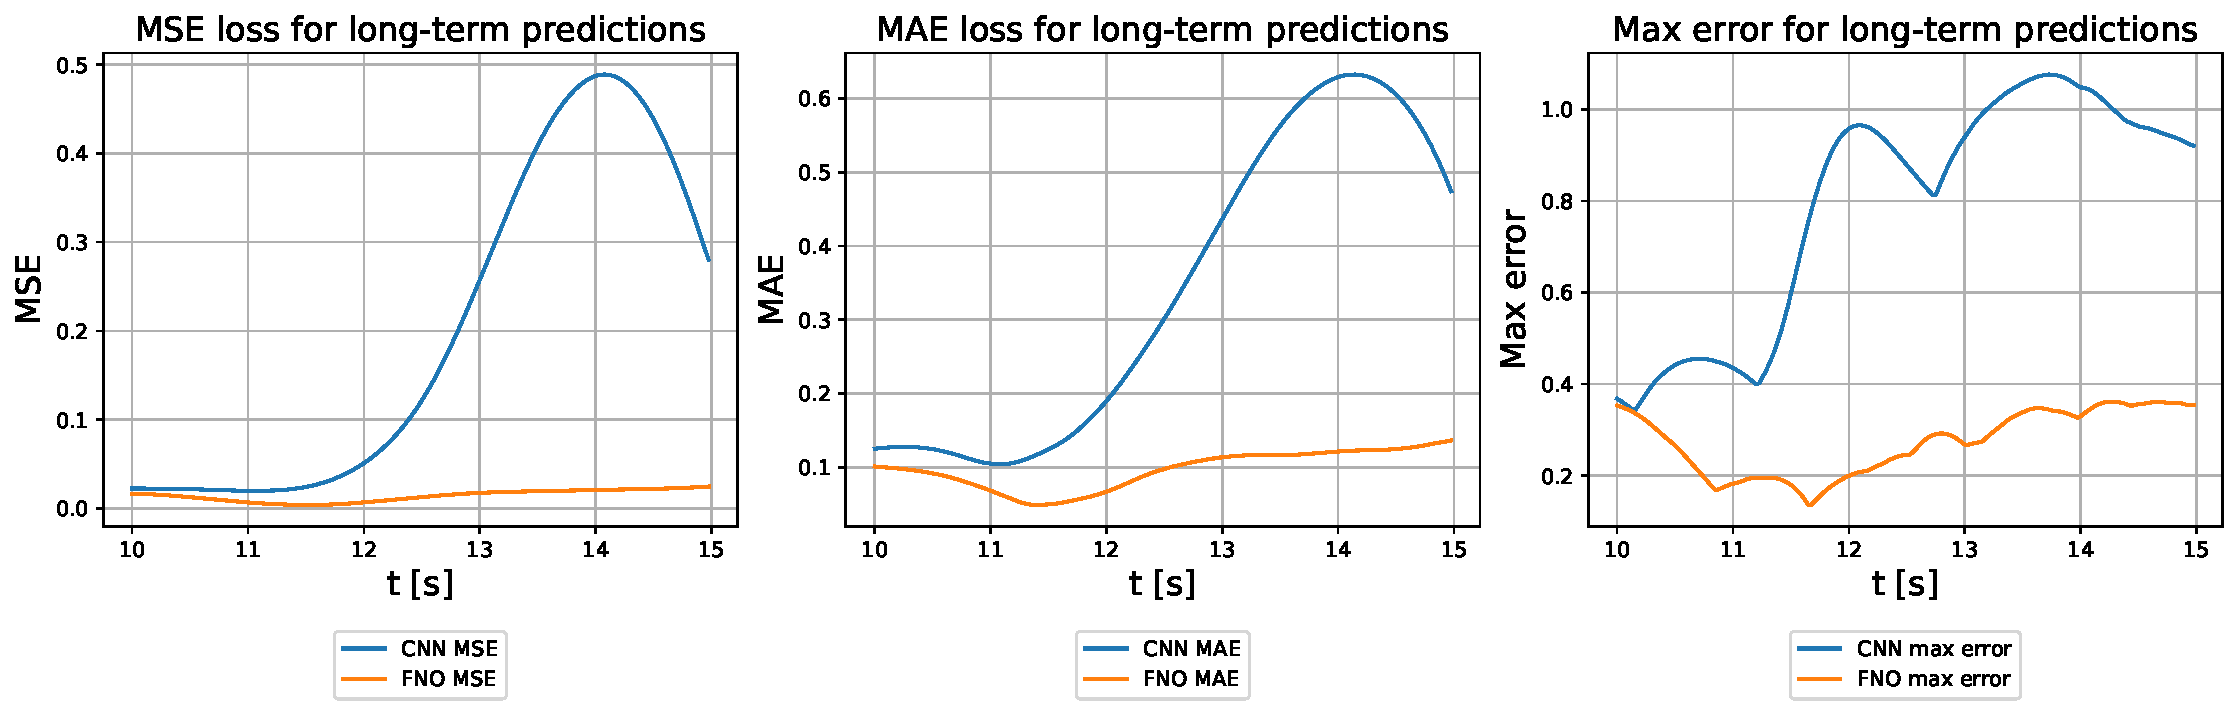
\includegraphics[width=0.99\textwidth]{C:/Users/Matteo/Shallow-Water-Equations/plots/2D_CNN_FNO_mse_mae_max_error.pdf}
    \caption{MSE, MAE and max error for the long-term predictions for the 2D CNN and FNO models.}\label{fig:2D_CNN_FNO_mse_mae_max_error}
\end{figure}
When making predictions, it is essential to consider the physical properties of the system, rather than relying solely on the loss functions.
The choice of error metric should align with the goals of the predictions.
For instance, it may be more important to minimize the MSE or the maximum absolute error, depending on the physical properties of the system.
This raises a key question: is it better to have one large error or many small errors?

As shown in \autoref{fig:2D_CNN_FNO_mse_mae_max_error}, the error increases as we make predictions further in time.
Overall, the FNO model demonstrates lower errors compared to the CNN model, indicating it may offer more accurate long-term predictions.











